% !TEX root = ../main.tex
\chapter{Implementation}
\label{Implementation}
In this section, how the design is implemented will be described in detail. 

\section*{Discrete Time Simulation Implementation Overview}
In the simulation, demand and generation requests are made and satisfied on a hourly basis. Due to the nature of Presage 2, actions and requests happen in discrete time steps. In this simulation, each hour has to be split into 5 discrete time-steps due to the parallel and random execution of actions and the discrete time nature of Presage 2. What actions are performed in each of the time steps are outlined below:
\begin{enumerate}
	\item During the first time step, Prosumer Agents submit their generation and demand requests to the Virtual Agent (Community) they are part of.
	\item During the second time step, Virtual Agents (Communities) aggregate the generation and demand requests received and submit their generation and demand requests to the Supervisor Agent.
	\item During the third time step, the Supervisor Agent gathers the total demand and generation requests and subsequently allocates the demand and generation to the Virtual Agents.
	\item During the fourth time step, the Virtual Agents (Communities) receive the allocation given by the supervisor, and allocates that appropriately to the Agents.
	\item During the 5th time step, the Agents appropriates the demand and generation allocation that has been given to them.
\end{enumerate}

\section*{Agent Class Structure and Implementation}
Agents in Presage 2 are created by extending the \textit{AbstractParticipant} class as shown in the \ac{UML} diagram in figure \ref{fig:AgentUML}. 

A Virtual Agent (\textit{ParentAgent} class) represents connected Prosumer Agents. It is required to:
\begin{itemize}
	\item Keep track of the Supervisor Agent, and communicate with it the group demand and generation requests
	\item Keep track of the Prosumer Agents that it is connected to and submit demand and generation requests on their behalf
	\item Submit generation and demand requests to the Supervisor Agent it is connected to
	\item Enforce demand and generation quotas on connected Prosumer Agents
\end{itemize}

To perform the duties outlined above, the following methods are implemented in the \textit{ParentAgent} class:
\begin{itemize}
	\item The \textit{constructor} of this object is responsible for keeping track of which Agent is the Supervisor Agent. The \textit{constructor} is called when this object is created in the initial Simulation set-up as part of the Agent creation and initialisation process.
	\item \textit{addChild()} method is used for keeping track of the Agents. This is also called during the initial Simulation set-up as part of the Agent creation and initialisation process.
	\item \textit{step(int)} method is called by Presage during the simulation to allow the Agent to act on the environment. demand and generation requests are sent to the supervisor, and allocation of demand and generation are also made to the Agents when this method is called automatically by Presage during a simulation.
\end{itemize}

The class \textit{MasterAgent} is how a Supervisor Agent is defined within the Simulator. As a special type of Virtual Agent, it extends from \textit{ParentAgent} class and is required to only do two things:
\begin{itemize}
	\item Keep track of the Virtual Agents in the community it is responsible for
	\item Allocating the correct amount of demand and generation to the Virtual Agents
\end{itemize}

To satisfy those requirements the following methods in the class are implemented:
\begin{itemize}
	\item \textit{addChild()} method is used for keeping track of the Virtual Agents. This is called during the initial Simulation set-up as part of the Agent creation and initialisation process.
	\item \textit{step(int)} method is called by Presage during the simulation to allow the Agent to act on the environment. Demand and generation are allocated to the Virtual Agents when this method is called automatically by Presage
\end{itemize}

Prosumer Agents are Virtual Agents but with no aggregation function, as a Prosumer Agent is the most elementary Agent is the most elementary Agent or sub-community in this holonic system simulation. A Prosumer Agent is required to:
\begin{itemize}
	\item Keep track of which Agent is the Virtual Agent
	\item Submit generation and demand requests to the Virtual Agent it is connected to
	\item Appropriate the allocated amount of generation and demand allocated
\end{itemize}

The Prosumer Agent is implemented with the following methods to allow it to perform the requirements outlined above:
\begin{itemize}
	\item The \textit{constructor} of this object is responsible for keeping track of which Agent is its \textit{ParentAgent}. The \textit{constructor} is called when this object is created in the initial Simulation set-up as part of the Agent creation and initialisation process.
	\item \textit{addChild()} method is used for keeping track of the Agents. This is called during the initial Simulation set-up as part of the Agent creation and initialisation process.
	\item \textit{step(int)} method is called by Presage during the simulation to allow the Agent to act on the environment. demand and generation requests are sent to the supervisor, and allocation of demand and generation are also made to the Agents when this method is called automatically by Presage.
	\item \textit{addProductivity(), addSocialUtility(), addProfileHourly()} are the methods that are called during the initial Simulation set-up as part of the Agent creation and initialisation process to define the properties of this Agent.
\end{itemize}


\begin{figure}[!h]
	\centering
	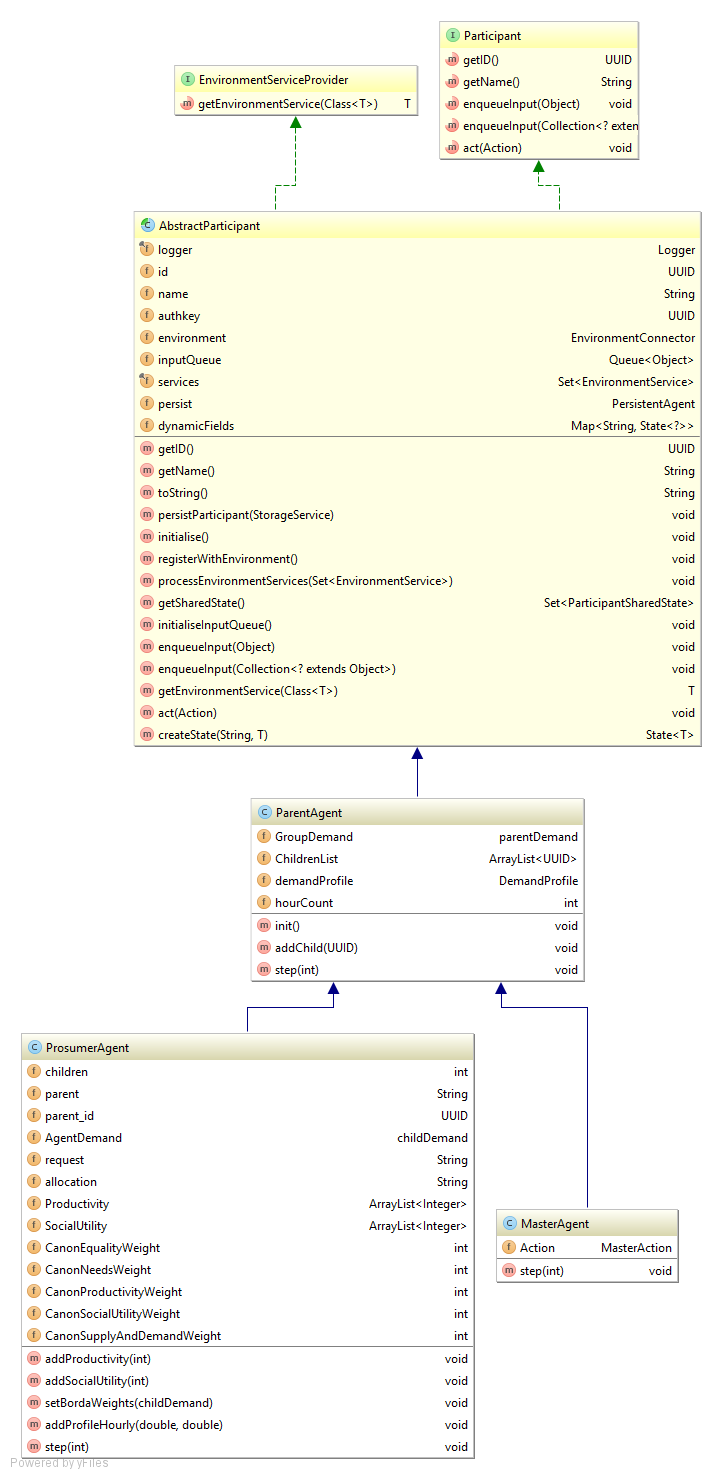
\includegraphics[scale=0.4]{Images/AgentUML.png}
	\caption{Agent UML Diagram}
	\label{fig:AgentUML}
\end{figure}

\clearpage

\section*{Demand Action}
Agents act on Environments and "Shared States" by performing \textit{Actions}. \textit{Actions} are implemented by extending the Java interface \textit{Action} from Presage 2. In the context of this simulation, an \textit{Action} would be a demand/generation request or a demand/generation allocation. As generation can be modeled as a negative demand, a single \textit{Action} such as the \textit{Demand Action} can be defined to represent both demand requests/quotas and generation requests/dispatch. \textit{childDemand} and \textit{parentDemand} are special instances of \textit{Demand}, and are responsible for representing demand/generation requests from Prosumer Agents and Virtual Agents respectively. The UML diagram of all of the \textit{Actions} in this simulation is defined in the UML diagram in figure \ref{fig:ActionUML}.

\begin{figure}[!h]
	\centering
	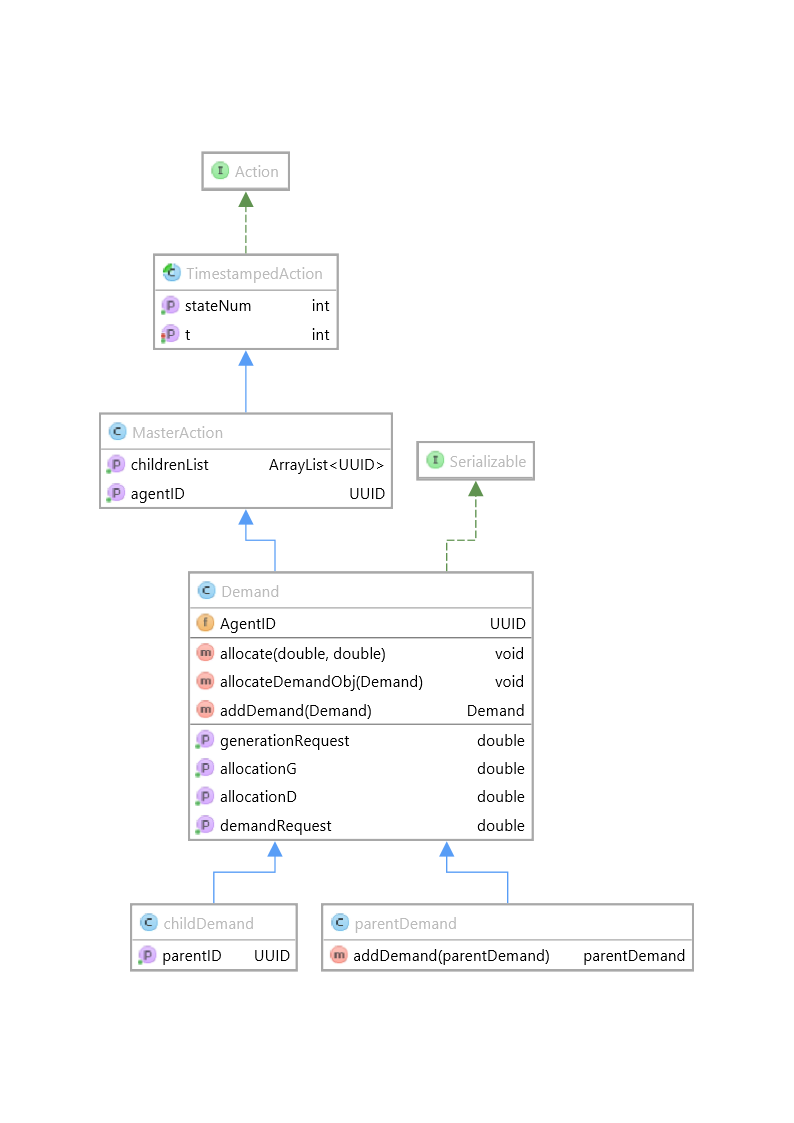
\includegraphics[scale=0.5]{Images/ActionUML.png}
	\caption{Actions UML Diagram}
	\label{fig:ActionUML}
\end{figure}

\section*{Action Handlers} % (fold)
\subsection*{Demand Handlers}
To enable the Environment to be able to process the Action requests, \textit{Action Handlers} need to be created to tell the simulation how to deal with Actions from Agents. In Presage 2, \textit{Action Handlers} are created by extending the implementing the Java interface \textit{ActionHandler}. The superclass \textit{Demand} isn't used by any of the Agents, so there are three \textit{Action Handlers}:  \textit{ChildDemandHandler}, \textit{ParentDemandHandler} and \textit{MasterActionHandler}. Depending on which the time step in the simulation hour it is, \textit{ChildDemandHandler} and \textit{ParentDemandHandler} \textit{Action Handlers} store or retrieve requests and allocations accordingly. The \textit{MasterActionHandler} is responsible for aggregating all demand and generation requests from all Virtual Agents and allocating that in time step 3. How these \textit{Action Handlers} relate to each other is described in the UML diagram in figure \ref{fig:ActionHandlerUML}. 

\subsection*{Master Action Handler}
A special case of the \textit{Action Handler} is the \textit{MasterActionHandler}. Unlike the other action handlers which access and data in one localised Environment Services, and methods in another Environment Service to allocate and st, this \textit{Action Handlers} is a \textit{Action-Environment Service} hybrid, which access and stores data in one localised Environment Service

\begin{figure}[!h]
	\centering
	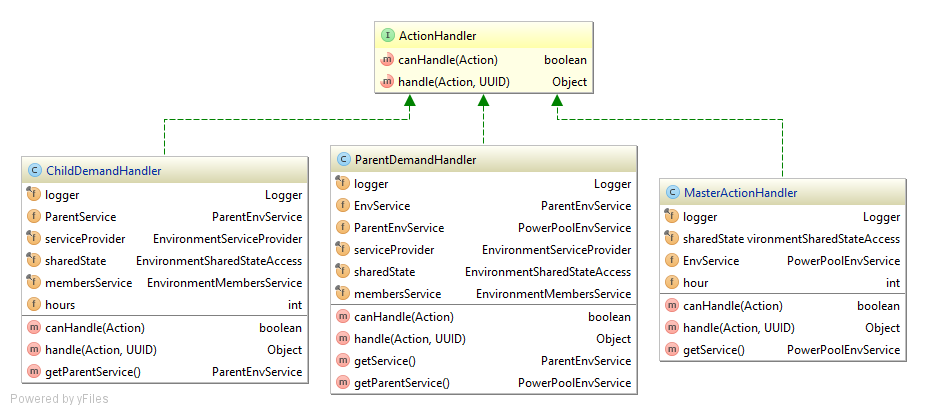
\includegraphics[scale=0.4]{Images/ActionHandlerUML.png}
	\caption{Action Handler UML Diagram}
	\label{fig:ActionHandlerUML}
\end{figure}
% subsubsection subsubsection_name (end)

\clearpage
\section*{Environment Services Implementation}
All Agents perform actions on Environments, which contains one or more "shared states". In Presage 2, all communication that happens between Agents are done via the environment by storing the data in a "shared state". In the context of this simulation, a "shared state" would be information such as demand and generation requests or the amount available in the Common Resource Pool. A visual diagram on how the Environment classes in this simulation are implemented can be found in figures \ref{fig:ServiceUML} and \ref{fig:ServiceUML2}.

\subsection*{Global Environment Service}
All Agents are registered to the Global Environment Service, defined by the \textit{GlobalEnvService} class. Like all Environment service classes in Presage, this was extended from the \textit{EnvironmentService} class built into Presage. This class contains all of the methods that are called when allocations are being made. During time step 3 of a simulated hour, the \textit{allocate()} method is called from the \textit{MasterActionHandler} to perform allocations on behalf of the Supervisor Agent. The demand and generation requests by all of the Virtual Agents are aggregated and stored in this Service. The \textit{allocate()} method by default satisfies all the requirements of connected Virtual Agents if there is enough generation to support it. If there is excess generation, the excess is curtailed proportionally. 
If however, there isn't enough generation, method \textit{allocate\_fairly()} is called, and the Virtual Agents are ranked according to the five applicable \textit{Rescher's Canons of Distributive Justice}. These rankings are computed by calling the methods such as \textit{canon\_of\_equality()} and the allocations are subsequently stored in the \textit{PowerPoolEnvService}.
At the end of the allocation process, the data about the allocation is stored in the environment ready for time step 3 of the next simulated hour via the method \textit{environmentStore}.

\begin{figure}[!h]
	\centering
	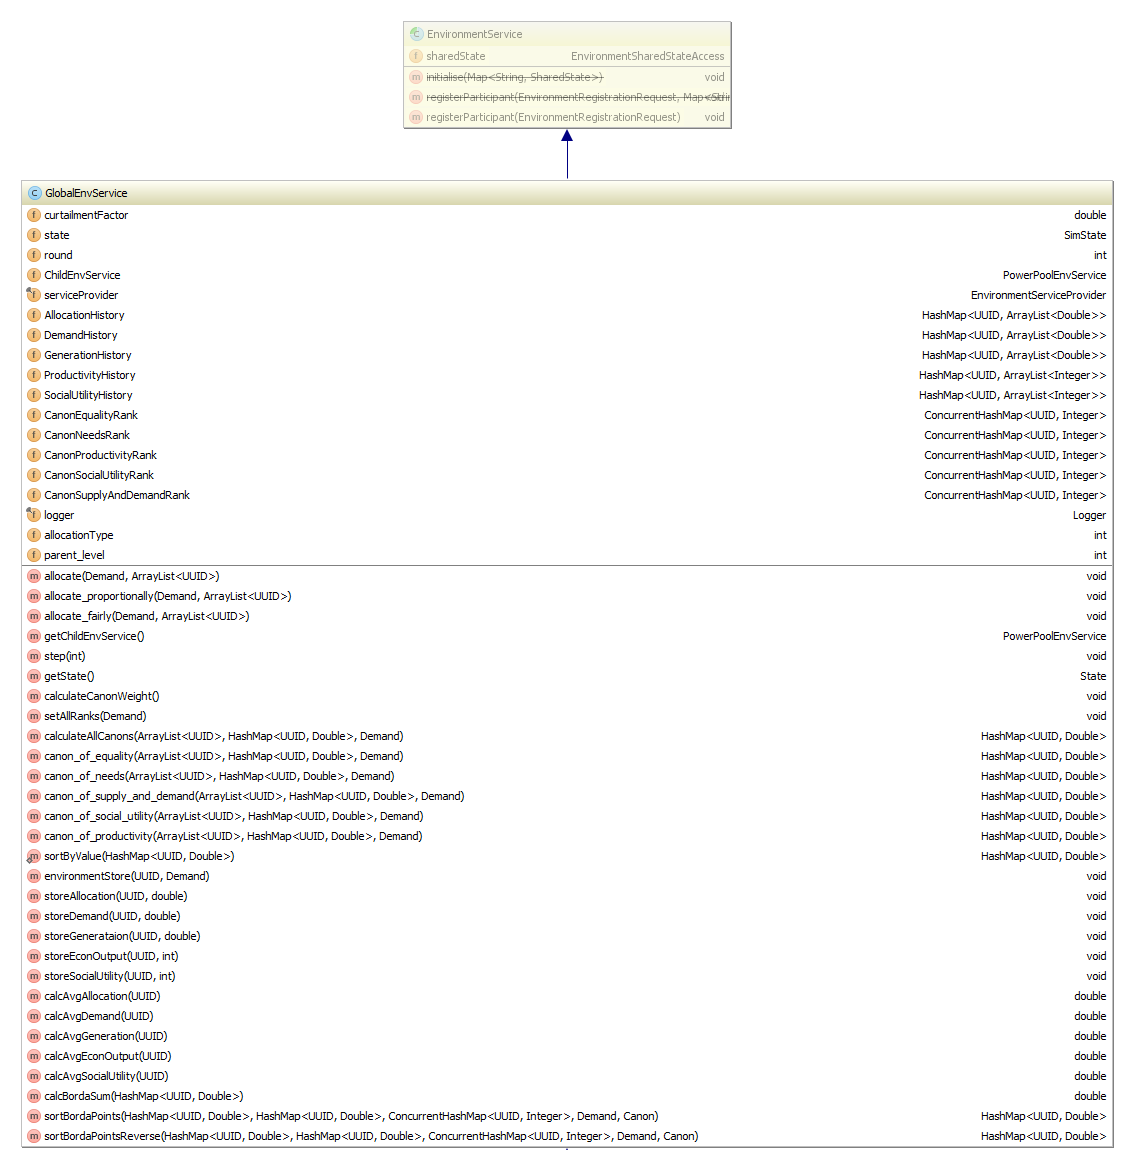
\includegraphics[scale=0.45]{Images/EnvironmentUML-1.png}
	\caption{Environment Services UML Diagram}
	\label{fig:ServiceUML}
\end{figure}

\subsection*{Supervisor Environment Service}
The \textit{PowerPoolEnvService} is the Environment Service accessible by both the Supervisor Agent and the Virtual Agents. The \textit{PowerPoolEnvService} extends the \textit{GlobalEnvService} class, and does a lot of the same things on a smaller scale. The \textit{PowerPoolEnvService} is used to store information about the Virtual Agents, such as their aggregated demand and generation requests, and contains the same methods that are called when allocations are being made by the Virtual Agents. During time step 2 of a simulated hour, Virtual Agents sum up their Prosumer Agent demand and generation requests, and store them in \textit{PowerPoolEnvService}. During time step 4 of a simulated hour, the \textit{allocate()} method is called from the \textit{parentDemandHandler}. \textit{allocate()} method by default satisfies all the requirements of Agents if there is enough generation to support it. If there is excess generation, the excess is curtailed proportionally. In a holonic system, Agents are not able to access information concerning other Agents that it is not directly connected to. A separate Environment Service is used to prevent the Supervisor Agent from being able to access and modify "shared states" about Prosumer Agents that are not directly connected to the Supervisor Agent.

Similar to the \textit{GlobalEnvService} class, if there isn't enough generation, method \textit{allocate\_fairly()} is called, and the Agents are ranked according to the five applicable \textit{Rescher's Canons of Distributive Justice}. These rankings are computed by calling the methods such as \textit{canon\_of\_equality()} which are inherited from the \textit{GlobalEnvService}. \textit{PowerPoolEnvService} contains "overriding" methods \textit{allocate()} and \textit{allocate\_fairly()} which do not inherit these from the \textit{GlobalEnvService}, as the allocation data is required to be stored in the \textit{ParentEnvService}. At the end of the allocation process, the data about the allocation is stored in the environment ready for time step 4 of the next simulated hour via the method \textit{environmentStore()}.

\begin{figure}[!h]
	\centering
	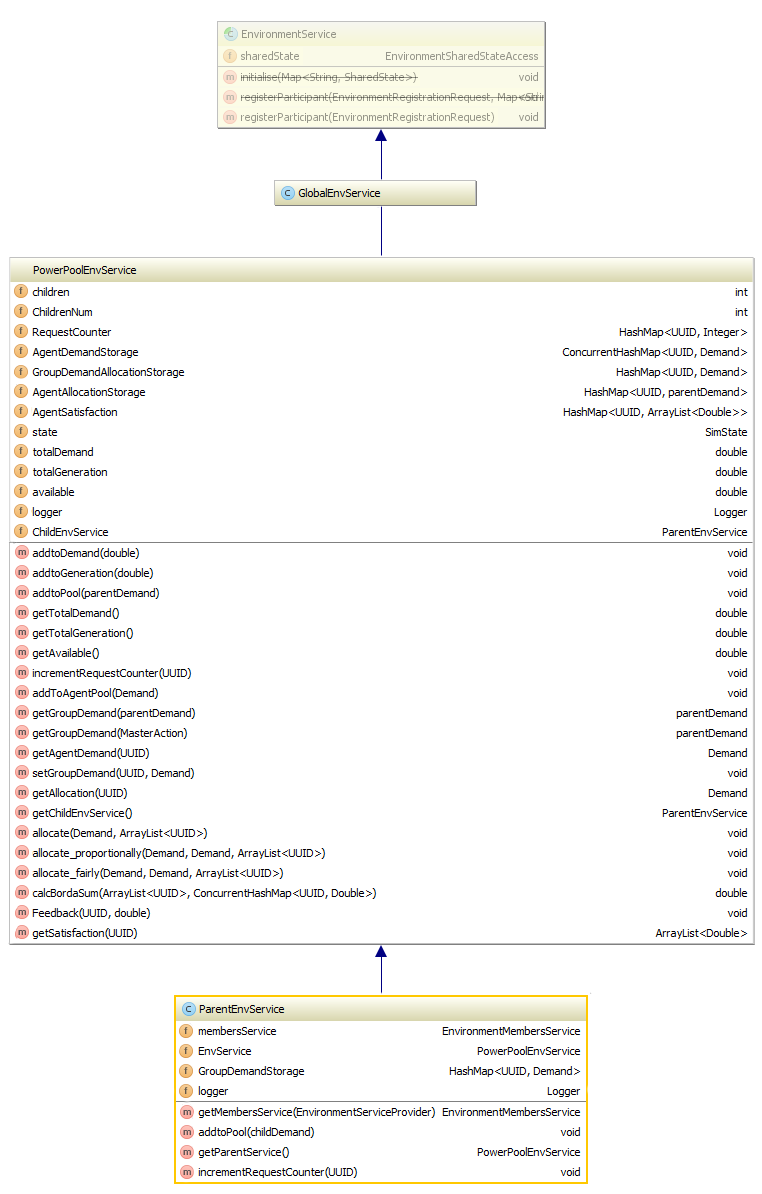
\includegraphics[scale=0.5]{Images/EnvironmentUML-2.png}
	\caption{Environment Services UML Diagram}
	\label{fig:ServiceUML2}
\end{figure}

\subsection*{Virtual Agent Environment Service}
The \textit{ParentEnvService} is the Environment Service accessible by both the Virtual Agents and the Prosumer Agents. The \textit{ParentEnvService} inherits from the \textit{PowerPoolEnvService}, and does the same things on a smaller scale. The \textit{ParentEnvService} is used to store information about the Prosumer Agents, such as their individual demand and generation requests, and also contain information about their allocations. During time step 1 of a simulated hour, Agents store their demand and generation requests in this Environment Service as a "shared state". During time step 2 of a simulated hour, Virtual Agents aggregate the stored demand and generation requests and store them in the \textit{PowerPoolEnvService}. During time step 5, Agents retrieve their allocations from the \textit{ParentEnvService}.

\section*{Setting up the simulation}
To set up the simulation with realistic demand and generation profiles, some measured data over a 24 hour period was used to set up the demand and generation profiles of the Agents. To simulate random and independent behaviour between Agents, each of the measured data points was randomly changed by 20\% according to a normal distribution centred around the data points. Figures \ref{fig:WindGenProfile}, \ref{fig:SolarGenProfile} and \ref{fig:DemandProfile} show a plot of the wind generation, solar generation and demand data used to set up the simulation.

\begin{figure} 
	\centering \newlength\figureheight \newlength\figurewidth 
	\setlength\figureheight{6cm} 
	\setlength\figurewidth{13cm} 
	% This file was created by matlab2tikz.
% Minimal pgfplots version: 1.3
%
%The latest updates can be retrieved from
%  http://www.mathworks.com/matlabcentral/fileexchange/22022-matlab2tikz
%where you can also make suggestions and rate matlab2tikz.
%
\definecolor{mycolor1}{rgb}{0.00000,0.44700,0.74100}%
%
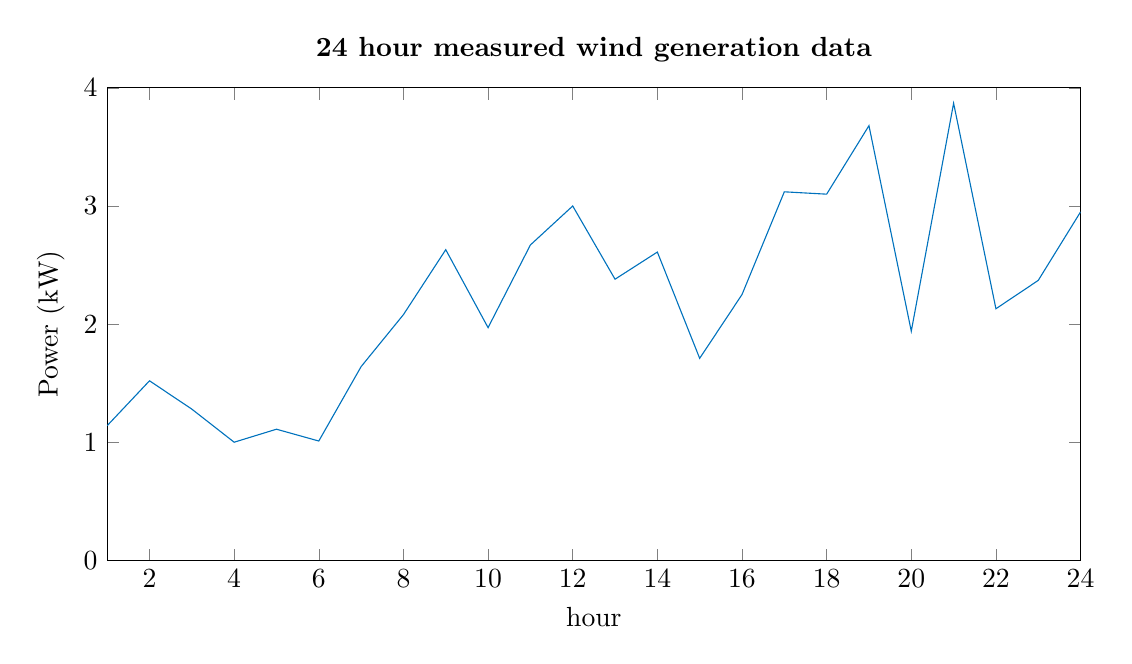
\begin{tikzpicture}

\begin{axis}[%
width=0.95092\figurewidth,
height=\figureheight,
at={(0\figurewidth,0\figureheight)},
scale only axis,
xmin=1,
xmax=24,
xlabel={hour},
ymin=0,
ymax=4,
ylabel={Power (kW)},
title style={font=\bfseries},
title={24 hour measured wind generation data}
]
\addplot [color=mycolor1,solid,forget plot]
  table[row sep=crcr]{%
1	1.14\\
2	1.52\\
3	1.28\\
4	1\\
5	1.11\\
6	1.01\\
7	1.64\\
8	2.08\\
9	2.63\\
10	1.97\\
11	2.67\\
12	3\\
13	2.38\\
14	2.61\\
15	1.71\\
16	2.25\\
17	3.12\\
18	3.1\\
19	3.68\\
20	1.94\\
21	3.87\\
22	2.13\\
23	2.37\\
24	2.95\\
};
\end{axis}
\end{tikzpicture}% 
	\caption{Wind Generation Profile} 
	\label{fig:WindGenProfile} 
\end{figure}

\begin{figure} 
	\centering
	\setlength\figureheight{6cm} 
	\setlength\figurewidth{13cm} 
	% This file was created by matlab2tikz.
% Minimal pgfplots version: 1.3
%
%The latest updates can be retrieved from
%  http://www.mathworks.com/matlabcentral/fileexchange/22022-matlab2tikz
%where you can also make suggestions and rate matlab2tikz.
%
\definecolor{mycolor1}{rgb}{0.00000,0.44700,0.74100}%
%
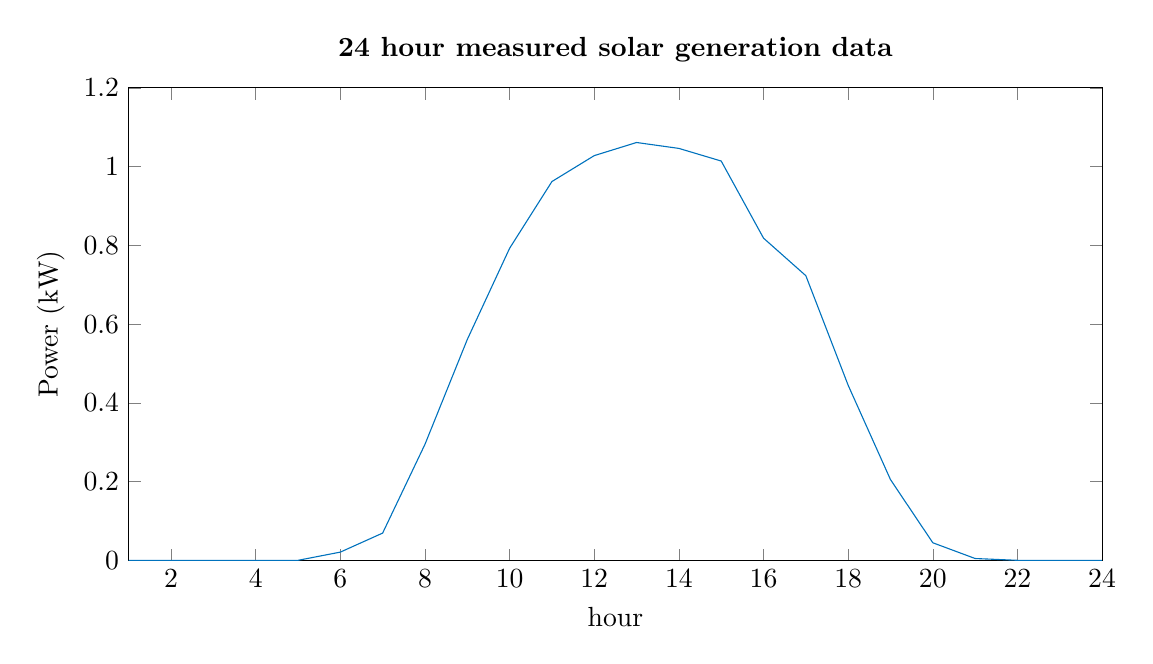
\begin{tikzpicture}

\begin{axis}[%
width=0.95092\figurewidth,
height=\figureheight,
at={(0\figurewidth,0\figureheight)},
scale only axis,
xmin=1,
xmax=24,
xlabel={hour},
ymin=0,
ymax=1.2,
ylabel={Power (kW)},
title style={font=\bfseries},
title={24 hour measured solar generation data}
]
\addplot [color=mycolor1,solid,forget plot]
  table[row sep=crcr]{%
1	0\\
2	0\\
3	0\\
4	0\\
5	0\\
6	0.020833333\\
7	0.069166667\\
8	0.294583333\\
9	0.560833333\\
10	0.7925\\
11	0.962083333\\
12	1.027916667\\
13	1.06125\\
14	1.04625\\
15	1.014166667\\
16	0.818333333\\
17	0.722916667\\
18	0.444583333\\
19	0.205\\
20	0.044583333\\
21	0.004583333\\
22	0\\
23	0\\
24	0\\
};
\end{axis}
\end{tikzpicture}% 
	\caption{Solar Generation Profile} 
	\label{fig:SolarGenProfile} 
\end{figure}

\begin{figure} 
	\centering
	\setlength\figureheight{6cm} 
	\setlength\figurewidth{13cm} 
	% This file was created by matlab2tikz.
% Minimal pgfplots version: 1.3
%
%The latest updates can be retrieved from
%  http://www.mathworks.com/matlabcentral/fileexchange/22022-matlab2tikz
%where you can also make suggestions and rate matlab2tikz.
%
\definecolor{mycolor1}{rgb}{0.00000,0.44700,0.74100}%
%
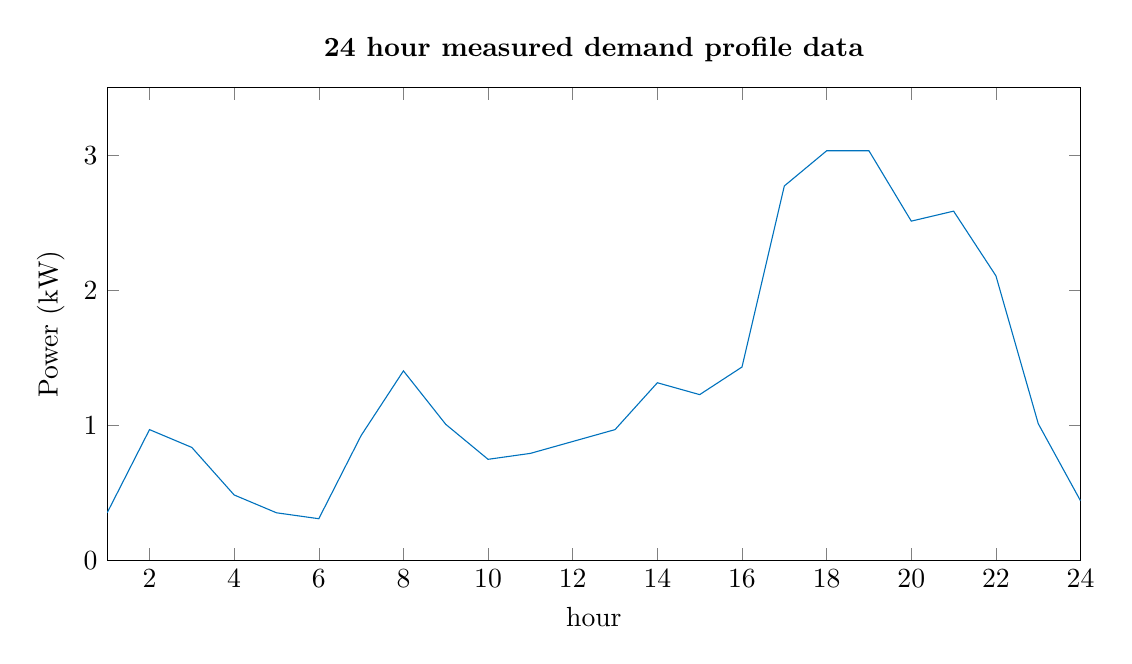
\begin{tikzpicture}

\begin{axis}[%
width=0.95092\figurewidth,
height=\figureheight,
at={(0\figurewidth,0\figureheight)},
scale only axis,
xmin=1,
xmax=24,
xlabel={hour},
ymin=0,
ymax=3.5,
ylabel={Power (kW)},
title style={font=\bfseries},
title={24 hour measured demand profile data}
]
\addplot [color=mycolor1,solid,forget plot]
  table[row sep=crcr]{%
1	0.35208\\
2	0.96822\\
3	0.83619\\
4	0.48411\\
5	0.35208\\
6	0.30807\\
7	0.92421\\
8	1.40343\\
9	1.00734\\
10	0.74817\\
11	0.79218\\
12	0.8802\\
13	0.96822\\
14	1.31541\\
15	1.22739\\
16	1.431975\\
17	2.773325\\
18	3.033875\\
19	3.033875\\
20	2.512775\\
21	2.58681\\
22	2.10759\\
23	1.01223\\
24	0.4401\\
};
\end{axis}
\end{tikzpicture}% 
	\caption{Demand Profile} 
	\label{fig:DemandProfile} 
\end{figure}

\section*{Issues}
Out of order parallel execution meant that Agents need to submit their individual demands to the SharedState, and have that summed at the end of each time step. It is not possible to sum the demands on the fly.

Being new to both Java and Presage presented problems of its own. It was difficult to understand how simulations could be run and therefore create our own. Some aspects of this project is similar to \textit{LPG'}, but due to API changes the code had to be redesigned and rewritten for this project.

One action per time step meant that it takes 5 time steps to simulate one round of request and appropriation of electricity. It would therefore take 24*4 time steps to simulate a full day of requests and appropriation.

Difficulty with initialising Agents with arrays meant that Agents had to be created with no demand or generation Profiles, and the demand and generation Profiles were added one by one by using the \textit{addProfileHourly()} method.